\chapter{Methodology}

\begin{document}
To illustrate the analysis methodology, we have a pipeline consisting of nine steps (Figure XX). First, we download npf\_train.csv dataset and explore the data. We remove the unnecessary columns, including 'id', 'date', and 'partlybad'. Next, we split the npf\_train.csv dataset into two parts, 80\% for training and 20\% for test sets using stratified sampling. After that, we standardize the features using Standardscaler, which normalizes data to mean = 0 and standard deviation = 1 by fitting the scaler on the training subset. This scaler is then applied to the test subset. As the number of features is too many, we reduce the dimension of our data by using principal component analysis (PCA). Similarly, we fit PCA on the training subset with 19 components as it captures 95\% of the variation and applies it to the test subset. At this stage, we have four datasets: training and test sets with original data, and training and test sets with PCA. 

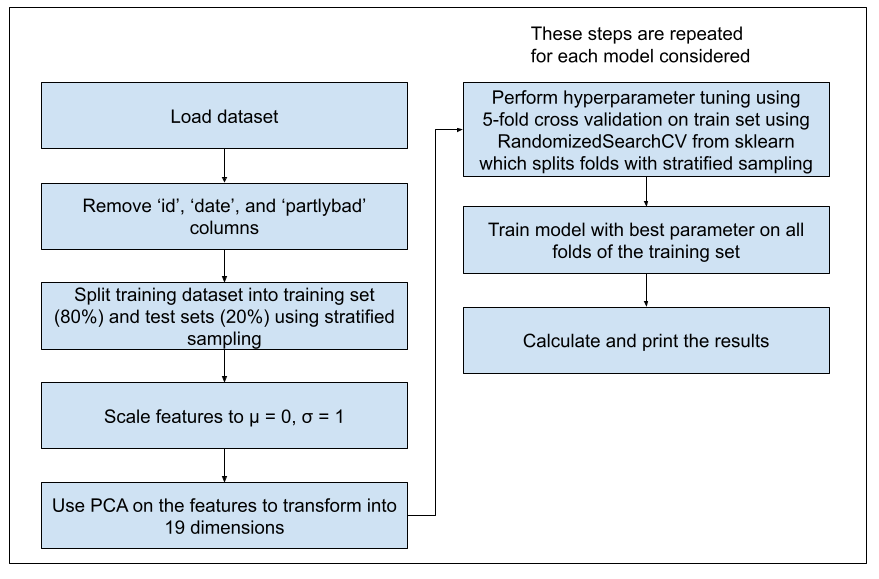
\includegraphics[scale=1.5]{pipeline}

The next step is to train the following generative and discriminative models on the datasets we have created.

\begin{enumerate}
    \item Generative model 
    
    The goal of generative models is to describe how data is created. The model relies on the Bayes theorem and uses parameters that maximizing the joint probability of P(X,Y) to trains a model.
    
    \begin{enumerate}
        \item NaiveBayes
        \item MLP classifier
    \end{enumerate}
    
    \item Discriminative model.
    
    The goal of discriminative models is to predicting the labels of the data. The model learns boundaries between classes in a dataset and trains a model using parameters that maximizing the conditional probability P(Y \textbar X).
    
    In each separate model, we set a 'class\_weight' parameter to 'balanced'. It will automatically assign class weights that are inversely proportionate to their relative frequencies.
    
    \begin{enumerate}
        \item Logistic Regression
        \item Logistic Regression - With Class Balanced Weights
        \item SVM
        \item SVM - With Class Balanced Weights
        \item Decision Tree
        \item Decision Tree - With Class Balanced Weights
        \item Random Forest
        \item Random Forest - With Class Balanced Weights
    \end{enumerate}
\end{enumerate}

For each model, we perform 5-fold cross-validation hyperparameter tuning. After that, the model with the best parameters is trained on train set and then evaluated on the test set for both original data and PCA.
\end{document}
